\subsection{Data processing frameworks}

The wide range of different receiver modes and setups has resulted in the development and propagation of common receiver software, spearheaded by NASA's \textit{Direct Readout Laboratory}, within a framework known as IPOPP (the International Planetary Observation Processing Package).
The software is open source and publicly distributed, meaning everyone from the official NASA ground station team through to smallest direct broadcast readout station can decode these satellite communications for their own purposes.

IPOPP follows a plugin-oriented architecture, in which existing command line programs for processing are packaged into system components with a common, configurable interface.
This enables the components to be assembled into pipelines for data processing through multiple stages.
The command line tools can also be used directly by end users for processing data obtained from the archives.

The pipeline for MODIS image decoding is outlined in Fig.~\textbf{TODO: ref}, showing that raw bytes from the attacker pass through multiple processing stages to convert the raw signal into processed, geographically tagged images.

Firstly, a QPSK demodulation stage processes the downconverted signal from the receiver into a raw byte sequence encoding the CADU frame structure.
Each CADU is processed through RT-STPS (Real Time \textbf{TODO: something}), which removes communications artefacts and outputs the demultiplexed byte sequences from inside the frames, which are intended to encode sequences of CCSDS packets for each instrument.

These byte sequences are stored for distribution and analysis on end user machines, and also passed on through multiple additional processing stages to extract the image data and geographically tag it.

\subsection{Secure handling of input data}

Since IPOPP and other downlink processing frameworks are handling potentially injected and untrusted user data, particular attention must be paid to areas of their architecture where user data is directly handled and parsed.
Ideally, these areas should be strictly separated from the core program control flow and, where implemented in a third party dependency, be patched and updated as vulnerabilities are discovered and mitigated.

In this work, we performed a security audit of the IPOPP plugins for MODIS image decoding to determine whether an attacker may be able to exploit the decoding system through overshadowing.

Unfortunately, the system appears to have been built with the assumption that downlinked data is benign at many different stages of the pipeline.
Many components fail to perform critical validation checks, passing malicious data through.
This enables an attacker to inject crafted data to target specific components, by crafting data to pass certain checks.

Once the bytes are at the desired component, an attacker can take advantage of the control flow of the program, which isn't cleanly separated from the code handling their input, to cause unintended consequences within the program.
Error handling code is often the least well tested, and the attacker can exploit this by purposefully making their packet fail certain checks.
Depending on the implementation, this may result in the rejection of the packet, denial of service through system crash, or potentially worse.
Finding such untested pathways is relatively easy due to the many disparate, stateful, and moving parts within the software.

An attacker may also choose to leverage known CVE-documented exploits which are present in the precompiled libraries distributed amongst the source code.
Several of additional these libraries have not been updated in a decade, yet directly parse the input data.




\begin{figure}
    \centering
    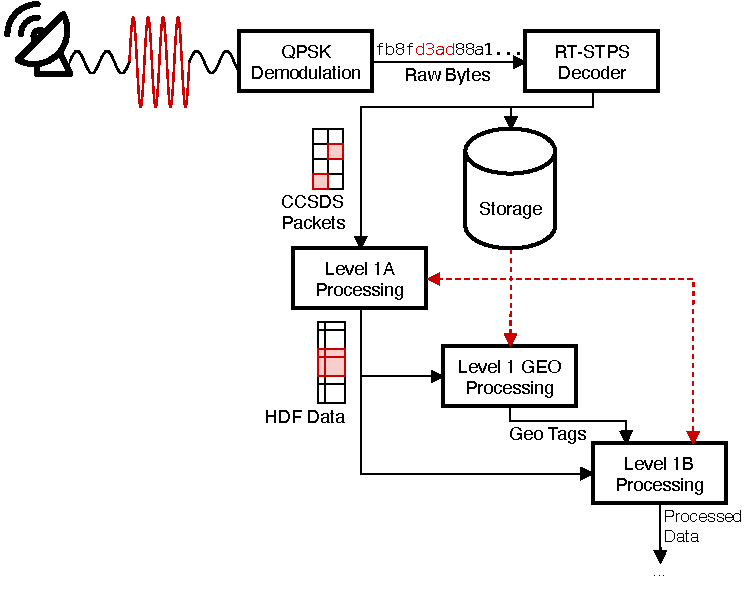
\includegraphics[width=\columnwidth]{diagrams/attack_flow.pdf}
    \caption{Flow of data through an EOS ground station and processing system. Attacker-injected data is highlighted in red. Manually-triggered reprocessing steps are indicated using dotted lines.}
    \label{fig:attack_flow}
\end{figure}

%Existing satellite systems often forego cryptographic means of verifying authenticity due to requirements of backwards compatibility and public availability.
%Therefore, the ground station programs for decoding, processing, and storing the data must be built with security in mind; particular attention must be paid to areas that directly handle and parse the incoming data.
%These areas should be strictly separated from the core program control flow and, where implemented in a third party dependency, be patched and updated as vulnerabilities are discovered and mitigated.

%The programs must also be tested relative to all of their possible configurations, rather than assuming a single golden path of execution.
%This is especially important if the software is intended to be run in different contexts, such as processing near real-time signals, and the reprocessing of stored data; the differing configurations may make otherwise inaccessible code paths now executable.
%In the worst case, this would allow the attacker, using only a transmitter near a satellite dish, to inject artefacts into public datasets that only cause malicious behaviour once reprocessed on an end user's machine.
